% Figure: prefill and decode evaluate the same conditional distribution
% p(x_t | x_{<t}) with opposite data-flow economics.  Design width ~168mm.
\documentclass[border=0pt]{standalone}
\usepackage{amsmath,amssymb}
% Shared visual language for the figures of the book.
% Every figure in this directory loads this file so the chapter reads as one system.
% NOTE: no blank lines are allowed inside \tikzset{...} (a blank line emits \par
% and breaks key scanning).
\NeedsTeXFormat{LaTeX2e}
\ProvidesPackage{figstyle}[2026/10/21 Figure style for Free Energy to LLMs]

\RequirePackage{tikz}
\usetikzlibrary{arrows.meta,positioning,calc,fit,shapes.geometric,shapes.misc,%
  backgrounds,matrix,decorations.pathreplacing,decorations.markings,patterns.meta}

% ---------------------------------------------------------------- palette
% Same values as book/preamble/style.tex, prefixed with F.
\definecolor{FNavy}{HTML}{14324A}
\definecolor{FTeal}{HTML}{0E7490}
\definecolor{FSky}{HTML}{E7F5F8}
\definecolor{FOrange}{HTML}{D97706}
\definecolor{FAmber}{HTML}{FFF3D6}
\definecolor{FInk}{HTML}{1F2937}
\definecolor{FSlate}{HTML}{64748B}
\definecolor{FMist}{HTML}{F5F7FA}
\definecolor{FRose}{HTML}{9F1239}
\definecolor{FRoseMist}{HTML}{FFF1F2}

% ---------------------------------------------------------------- semantics
% Teal   = probability / model / data object
% Orange = training objective, cost, or the quantity moved through the system
% Navy   = neutral structure
% Slate  = secondary label or metadata
% Rose   = failure mode, hazard, masked-out region
\tikzset{
  % Lay figures out in millimetres.  A figure designed 168mm wide is included at
  % \textwidth, so its fonts appear at exactly the size written here.
  every picture/.style={x=1mm,y=1mm,font=\small,line cap=round,line join=round},
  % ---- block styles
  nbase/.style={draw,rounded corners=1.2pt,align=center,inner sep=2.4pt,%
    minimum height=7mm,text=FInk},
  nteal/.style={nbase,draw=FTeal,fill=FSky},
  norange/.style={nbase,draw=FOrange,fill=FAmber},
  nnavy/.style={nbase,draw=FNavy,fill=white},
  nsoft/.style={nbase,draw=FSlate!55,fill=FMist},
  nrose/.style={nbase,draw=FRose,fill=FRoseMist},
  ghost/.style={draw=none,fill=none,align=center,inner sep=1pt},
  plain/.style={draw=none,fill=none,align=center,inner sep=0pt},
  % ---- arrows
  ar/.style={-{Latex[length=1.7mm,width=1.35mm]},draw=FSlate,line width=0.75pt},
  ard/.style={ar,dashed},
  arteal/.style={ar,draw=FTeal},
  arorange/.style={ar,draw=FOrange},
  arrose/.style={ar,draw=FRose},
  thickar/.style={ar,line width=1.2pt},
  % ---- text roles
  ftitle/.style={font=\large\bfseries,text=FNavy,align=center},
  ptitle/.style={font=\small\bfseries,text=FNavy,align=center},
  ptitleo/.style={font=\small\bfseries,text=FOrange,align=center},
  lbl/.style={font=\scriptsize,text=FSlate,align=center,inner sep=1pt},
  lblt/.style={lbl,text=FTeal},
  lblo/.style={lbl,text=FOrange},
  lbln/.style={lbl,text=FNavy},
  lblr/.style={lbl,text=FRose},
  sub/.style={font=\scriptsize,text=FSlate!90,align=center,inner sep=1pt},
  monob/.style={font=\ttfamily\scriptsize,text=FInk,inner sep=1pt},
  mathb/.style={font=\small,text=FInk,inner sep=1pt},
  eqn/.style={font=\scriptsize,inner sep=1.5pt,text=FInk},
  % ---- decorations
  brace/.style={decorate,decoration={brace,amplitude=2.4pt},draw=FSlate,%
    line width=0.6pt},
  bracet/.style={brace,draw=FTeal},
  braceo/.style={brace,draw=FOrange},
  axis/.style={draw=FSlate!55,line width=0.6pt},
  guide/.style={draw=FSlate!45,line width=0.5pt,dashed},
  halolabel/.style={font=\scriptsize,text=FInk,fill=white,fill opacity=0.85,%
    text opacity=1,inner sep=1.4pt,align=center},
}

% Figure title above the drawing, anchored at the figure's top-left.
\newcommand{\figtitle}[2][0]{%
  \node[ftitle,anchor=north west,outer sep=0pt] at (#1,0) {#2};}

% Rounded panel behind a subgroup of nodes.
\newcommand{\figpanel}[3][]{%
  \node[draw=FSlate!35,fill=#3,rounded corners=2pt,inner sep=2.6mm,#1] {#2};}

\endinput

\begin{document}
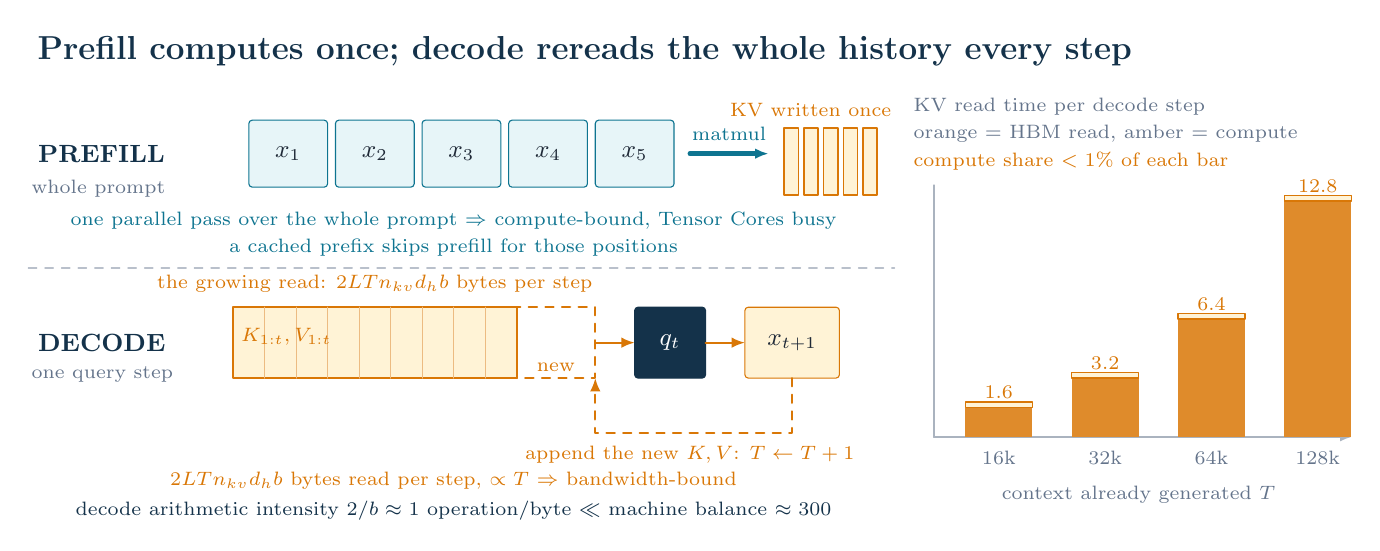
\begin{tikzpicture}
\figtitle{Prefill computes once; decode rereads the whole history every step}
% ------------------------------------------------------------------ prefill
\node[ptitle,anchor=west] at (0,-16) {PREFILL};
\node[lbl,anchor=west] at (0,-20.5) {whole prompt};
\foreach \i/\c in {1/33,2/44,3/55,4/66,5/77}{%
  \node[nteal,minimum width=10mm,minimum height=8.5mm,inner sep=0pt] at (\c,-16) {$x_{\i}$};}
\draw[arteal,line width=1.6pt] (84,-16)--(94,-16);
\node[lblt] at (89,-13.5) {matmul};
\foreach \q in {96,98.5,101,103.5,106}{%
  \draw[fill=FAmber,draw=FOrange,line width=0.6pt] (\q,-21.25) rectangle ++(1.8,8.5);}
\node[lblo,anchor=east] at (110,-10.4) {KV written once};
\node[lblt] at (54,-24.5)
  {one parallel pass over the whole prompt $\Rightarrow$ compute-bound, Tensor Cores busy};
\node[lblt] at (54,-28)
  {a cached prefix skips prefill for those positions};
\draw[guide] (0,-30.5)--(110,-30.5);
% ------------------------------------------------------------------- decode
\node[ptitle,anchor=west] at (0,-40) {DECODE};
\node[lbl,anchor=west] at (0,-44) {one query step};
\node[lblo] at (44,-32.5)
  {the growing read: $2LTn_{kv}d_hb$ bytes per step};
\draw[fill=FAmber,draw=FOrange,line width=0.75pt] (26,-44.5) rectangle (62,-35.5);
\foreach \q in {30,34,38,42,46,50,54,58}{%
  \draw[draw=FOrange!50,line width=0.4pt] (\q,-44.5)--(\q,-35.5);}
\draw[draw=FOrange,dashed,line width=0.75pt] (62,-44.5) rectangle (72,-35.5);
\node[lblo,anchor=west] at (26.6,-39.3) {$K_{1:t},V_{1:t}$};
\node[lblo] at (67,-43.1) {new};
\draw[arorange] (72,-40)--(77,-40);
\node[draw=FNavy,fill=FNavy,text=white,rounded corners=1.2pt,minimum width=9mm,%
  minimum height=9mm,inner sep=0pt] at (81.5,-40) {$q_t$};
\draw[arorange] (86,-40)--(91,-40);
\node[norange,minimum width=12mm,minimum height=9mm,inner sep=0pt] at (97,-40) {$x_{t+1}$};
\draw[arorange,dashed] (97,-44.5)--(97,-51.5)--(72,-51.5)--(72,-44.5);
\node[lblo,anchor=north] at (84,-52.7) {append the new $K,V$: $T\leftarrow T+1$};
\node[lblo] at (54,-57.5)
  {$2LTn_{kv}d_hb$ bytes read per step, $\propto T$ $\Rightarrow$ bandwidth-bound};
\node[lbln] at (54,-61.3)
  {decode arithmetic intensity $2/b\approx1$ operation/byte $\ll$ machine balance $\approx300$};
% ------------------------------------------------------- quantitative payoff
\node[lbl,anchor=west] at (112,-10) {KV read time per decode step};
\node[lbl,anchor=west] at (112,-13.5) {orange = HBM read, amber = compute};
\node[lblo,anchor=west] at (112,-17) {compute share $<1\%$ of each bar};
\draw[axis] (115,-52)--(115,-20);
\draw[axis,-{Latex[length=1.4mm,width=1.1mm]}] (115,-52)--(168,-52);
\foreach \bx/\bh/\bl/\bm in {119/3.75/16k/1.6,132.5/7.5/32k/3.2,146/15/64k/6.4,159.5/30/128k/12.8}{%
  \draw[fill=FOrange!85,draw=none] (\bx,-52) rectangle ++(8.5,\bh);%
  \draw[fill=FAmber,draw=FOrange,line width=0.5pt] (\bx,-52+\bh) rectangle ++(8.5,0.7);%
  \node[lbl,anchor=north] at (\bx+4.25,-53.3) {\bl};%
  \node[lblo,anchor=south] at (\bx+4.25,-51.3+\bh) {\bm};}
\node[lbl,anchor=north] at (141,-57.8) {context already generated $T$};
\end{tikzpicture}
\end{document}
